\begin{frame}{Giới thiệu}
    Sự dễ tổn thương của DNNs
    \begin{figure}
    \centering
    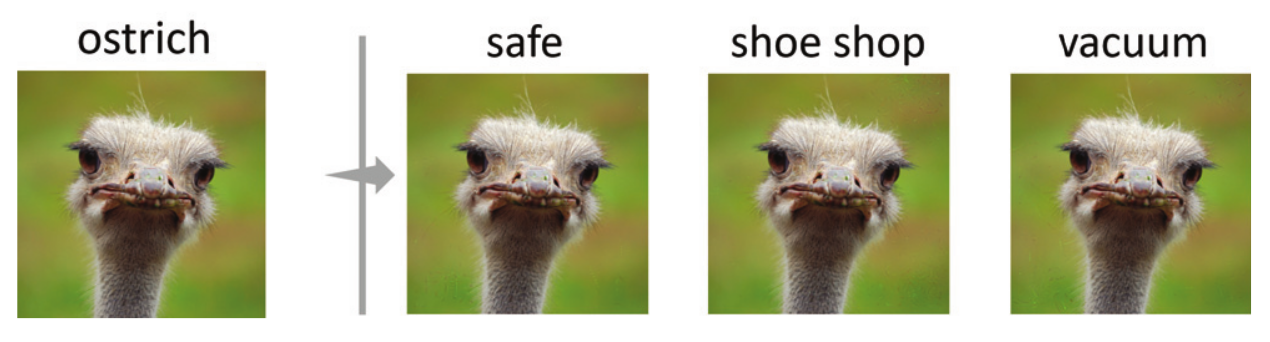
\includegraphics[scale=0.2]{images/fig_01.png}
    \caption{Các mẫu đối nghịch bị phân loại sai
        bởi mô hình Inception-V3}
    \end{figure}
\end{frame}

\begin{frame}{Giới thiệu - Các loại tấn công}
    \begin{enumerate}
        \item Tấn công nhắm đích - \textit{targeted attacks}
        \item Tấn công không nhắm đích - \textit{untargeted attacks}
    \end{enumerate}
\end{frame}

\begin{frame}{Giới thiệu: Huấn luyện đối nghịch}
    Huấn luyện đối nghịch (\textit{adverarial training}) (Madry et al. 2017): Sử dụng mẫu đối nghịch để huấn luyện một mô hình mạnh có khả năng chống chịu với các nhiễu của mẫu đối nghịch.
\end{frame}

\begin{frame}{Giới thiệu: Tấn công phân loại ảnh}
    \begin{enumerate}
        \item Tấn công phân loại ảnh dựa trên mạng neuron tích chập
        \item Mẫu đối nghịch được tạo ra để làm sai lệch kết quả phân loại
        \item Mẫu mới được tạo ra (gần) giống với mẫu gốc
    \end{enumerate}
\end{frame}

\begin{frame}{Giới thiệu: Độ nhiễu}
    $\lVert x \rVert_q = \left( \sum_{i=1}^p |x_i|^q \right)^{\frac{1}{q}}$ kí hiệu chuẩn $L_q$
    của vector $p$ chiều $x = [x_1, ..., x_p]$ với $q \geq 1$ 
    
    \begin{itemize}
        \item $L_{\infty}$: Đánh giá sự thay đổi tối đa các pixel (oodfellow, Shlens, and Szegedy 2015)
        \item $L_2$: Cải thiện chất lượng hình ảnh (Carlini and Wagner 2017b)
        \item $L_1$: Sử dụng trong các bài toán phục hồi ảnh (Fu et al. 2006)
    \end{itemize}

    \textit{Trong bài toán mẫu đối nghịch, độ biến dạng $L_1$ đánh giá tổng các thay đổi trong nhiễu loạn và đóng vai trò là một thành phần
    (hàm) lồi đo lường số lượng pixel thay đổi (độ thưa) gây ra bởi nhiễu}
\end{frame}

\begin{frame}{Giới thiệu - Các tập dữ liệu thử nghiệm}
    Tấn công dựa trên $L_1$ với các tập dữ liệu  
    \begin{itemize}
        \item MNIST
        \item CIFAR-10
        \item ImageNet
    \end{itemize}
    Được so sánh với các tấn công dựa trên $L_2$ và $L_{\infty}$
\end{frame}